\documentclass[12pt, a4paper, oneside]{book}
\usepackage[hidelinks]{hyperref}
\usepackage[slovak]{babel}
\usepackage{epsfig}
\usepackage{epstopdf}
\usepackage[chapter]{algorithm}
\usepackage{algorithmic}
\usepackage{listings}
\usepackage{amsmath}
\usepackage{amssymb}
\usepackage{graphicx}
\usepackage{multirow}
\usepackage{color}
\usepackage{url}
\usepackage[utf8]{inputenc}
\usepackage[T1]{fontenc}
\usepackage{setspace}
\usepackage{tabularx}
\usepackage{textcomp}
\usepackage{caption}
\usepackage{natbib}

% TODO NOTES
\usepackage{todonotes}
%\usepackage[disale]{todonotes}
\usepackage{xcolor}
\usepackage[normalem]{ulem}
\usepackage{soul}

%%% TODO Notes
\newcommand{\assignment}[2][]{\todo[caption={},inline,bordercolor=green!67!yellow!75!black!50,color=green!67!yellow!25,size=\footnotesize,#1]{#2}}
\newcommand{\overview}[2][]{\todo[caption={},inline,color=blue!85!green!25,bordercolor=blue!85!green!50!black!50,size=\footnotesize,#1]{#2}}
\newcommand{\minor}[2][]{\todo[caption={},color=gray!30,bordercolor=gray,inline,size=\footnotesize,#1]{#2}}
\newcommand{\cutting}[2][]{\todo[color=yellow!30,bordercolor=yellow!50!black!50,inline,size=\footnotesize,#1]{#2}}
\newcommand{\bigassignment}[2][]{\todo[inline, caption={Big assignment},
    color=green!40, #1]{\begin{minipage}{\textwidth-4pt}#2\end{minipage}}}
\newskip\movedskip
\newcommand{\movespaceafter}[1]{%
    \movedskip=0pt%
    \ifhmode\ifdim\lastskip=0pt\else\movedskip=\lastskip\unskip\fi\fi
    #1\ifdim\movedskip=0pt\else\hskip\movedskip\fi
    \ignorespaces}
\newcommand{\reviewnote}[3][]{%
  \movespaceafter{\todo[inline,color=yellow!75!white,linecolor=yellow!85!black,#1]
      {\textsf{\bfseries Review #2:} \ignorespaces#3\par}}%
}
%\newcommand{\comment}[3][]{%
%  \movespaceafter{\todo[color=green!40,#1]
%      {\textsf{\bfseries #2:} \ignorespaces#3\par}}%
%}

\definecolor{mossgreen}{HTML}{146614}
\newcommand{\del}[1]{\color{red}\sout{#1}\color{black}\@}
\newcommand{\ins}[1]{\color{mossgreen}\uwave{#1}\color{black}\@}
\newcommand{\sug}[2]{\del{#1}\ins{#2}}

\newcommand{\UP}{$\uparrow$}
\newcommand{\DOWN}{$\downarrow$}
\newcommand{\UD}{$\updownarrow$}




\setstretch{1.5}
%\renewcommand\baselinestretch{1.5} % riadkovanie jeden a pol

% pekne pokope definujeme potrebne udaje
\newcommand\mftitle{Sémantické publikovanie spravodajských dát}
\newcommand\mftitlen{o bezpečnostných hrozbách}
\newcommand\mfthesistype{Diplomová práca}
\newcommand\mfauthor{Bc. Matej Rychtárik}
\newcommand\mfadvisor{doc. RNDr. Martin Homola, PhD.}
\newcommand\mfplacedate{Bratislava, 2021}
\newcommand\mfuniversity{UNIVERZITA KOMENSKÉHO V BRATISLAVE}
\newcommand\mffaculty{FAKULTA MATEMATIKY, FYZIKY A INFORMATIKY}
\newcommand{\sub}[1]{$_{\text{#1}}$}
\newcommand{\reference}[1]{č.~\ref{#1}}
\newcommand{\imageHeight}{150px}

\ifx\pdfoutput\undefined\relax\else\pdfinfo{ /Title (\mftitle) /Author (\mfauthor) /Creator (PDFLaTeX) } \fi

\begin{document}

\frontmatter

\thispagestyle{empty}

\noindent
\begin{minipage}{\textwidth}
\begin{center}
\textbf{\mfuniversity \\
\mffaculty}
\end{center}
\end{minipage}

\vfill
\begin{figure}[!hbt]
	\begin{center}
		
\includegraphics{images/logo_fmph}
		\label{img:logo}
	\end{center}
\end{figure}
\begin{center}
	\begin{minipage}{0.8\textwidth}
		\centerline{\textbf{\Large\MakeUppercase{\mftitle}}}
		\smallskip
		\centerline{\mfthesistype}
	\end{minipage}
\end{center}
\vfill
2021 \hfill
\mfauthor
\eject 
% koniec obalu

\thispagestyle{empty}

\noindent
\begin{minipage}{\textwidth}
\begin{center}
\textbf{\mfuniversity \\
\mffaculty}
\end{center}
\end{minipage}

\vfill
\begin{figure}[!hbt]
\begin{center}

\includegraphics{images/logo_fmph_dark}
\label{img:logo_dark}
\end{center}
\end{figure}
\begin{center}
\begin{minipage}{0.8\textwidth}
\centerline{\textbf{\Large\MakeUppercase{\mftitle}}}
\smallskip
\centerline{\mfthesistype}
\end{minipage}
\end{center}
\vfill
\begin{tabular}{l l}
%Registration number: & 40a99bd8-3cb6-4534-9330-c7fd9b5e5ca4 \\
Študijný program: & Aplikovaná informatika\\
Študijný odbor: & 2511 Aplikovaná informatika\\
Školiace pracovisko: & Katedra aplikovanej informatiky\\
Školiteľ: & \mfadvisor
\end{tabular}
\vfill
\noindent
\mfplacedate \hfill
\mfauthor
\eject 
% koniec titulneho listu

%\thispagestyle{empty}
%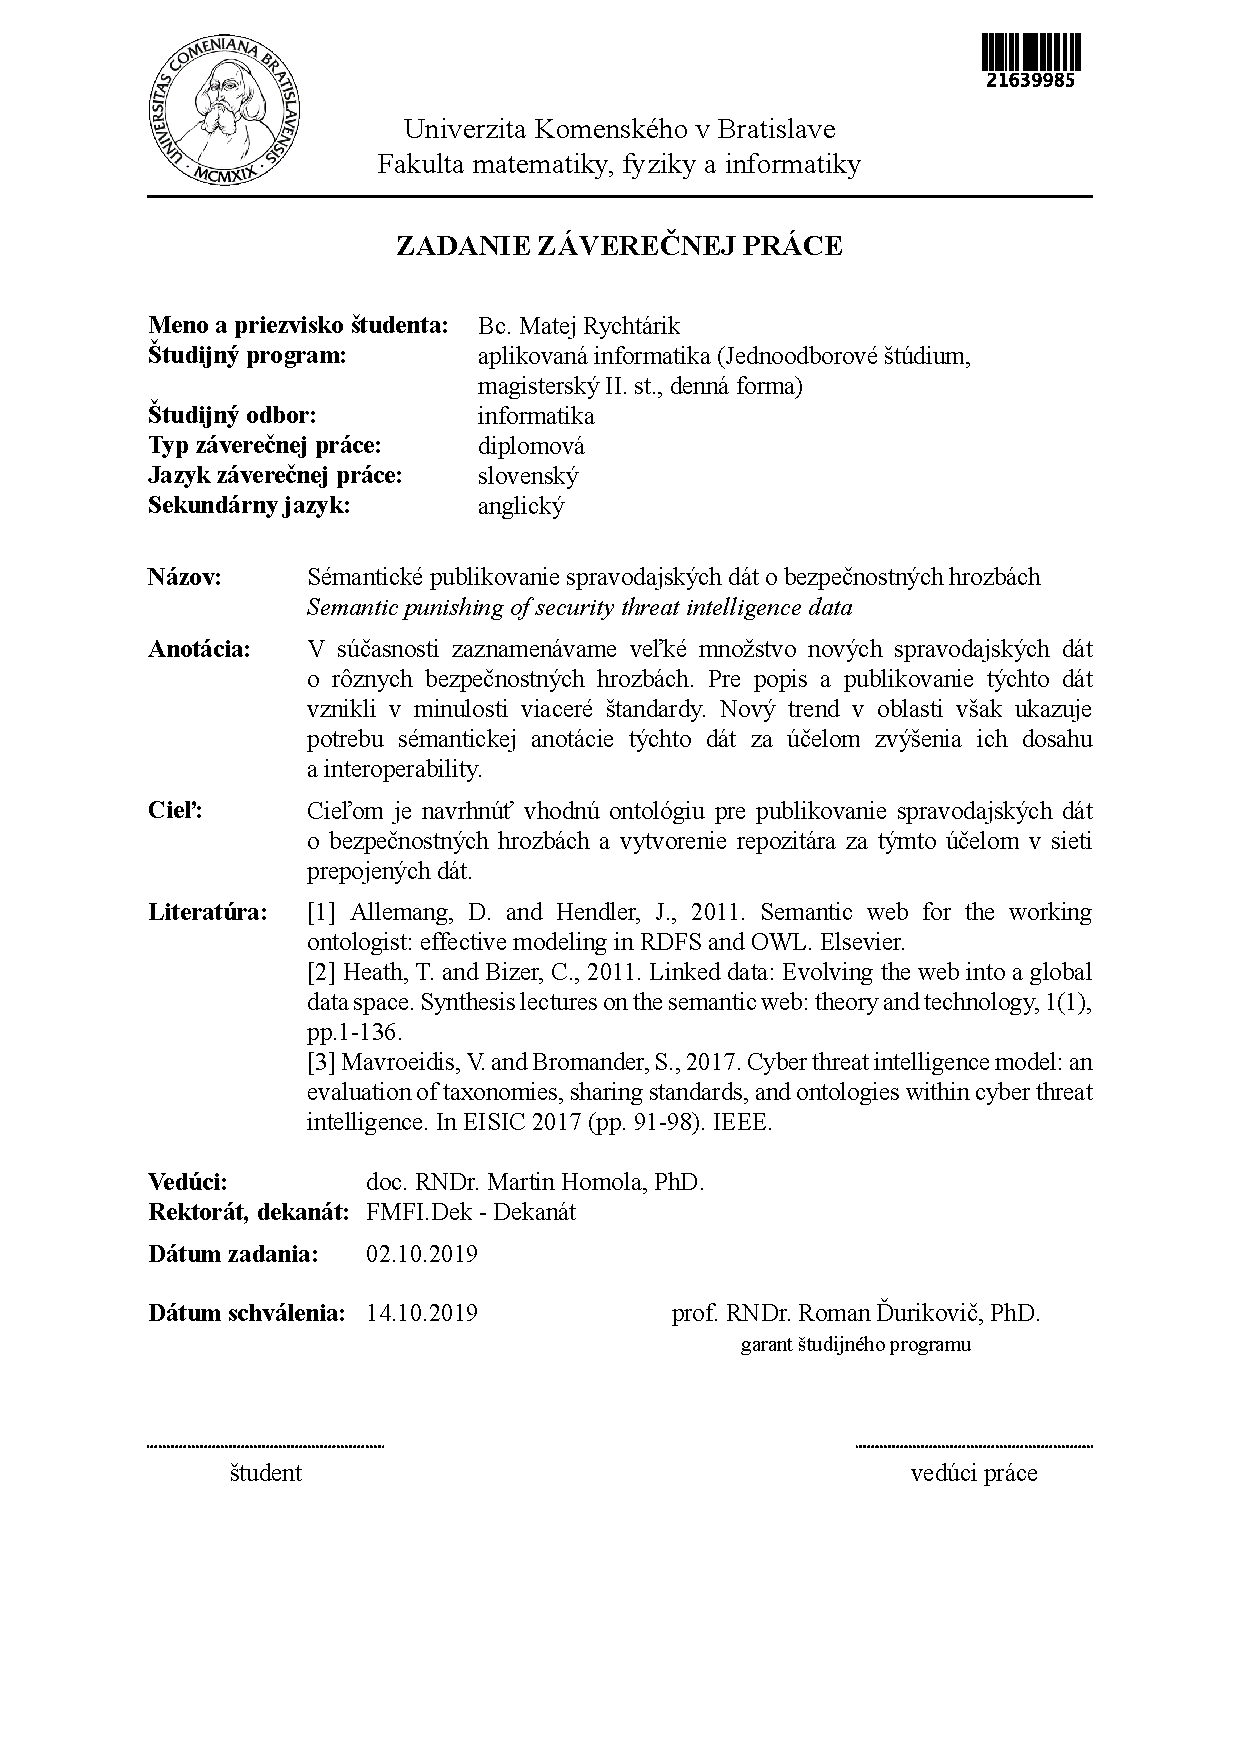
\includegraphics[width=\textwidth]{images/zadanie}
%\vfill
%\eject
% koniec zadania

\thispagestyle{empty}


\begin{figure}[H]
\begin{center}
\makebox[\textwidth]{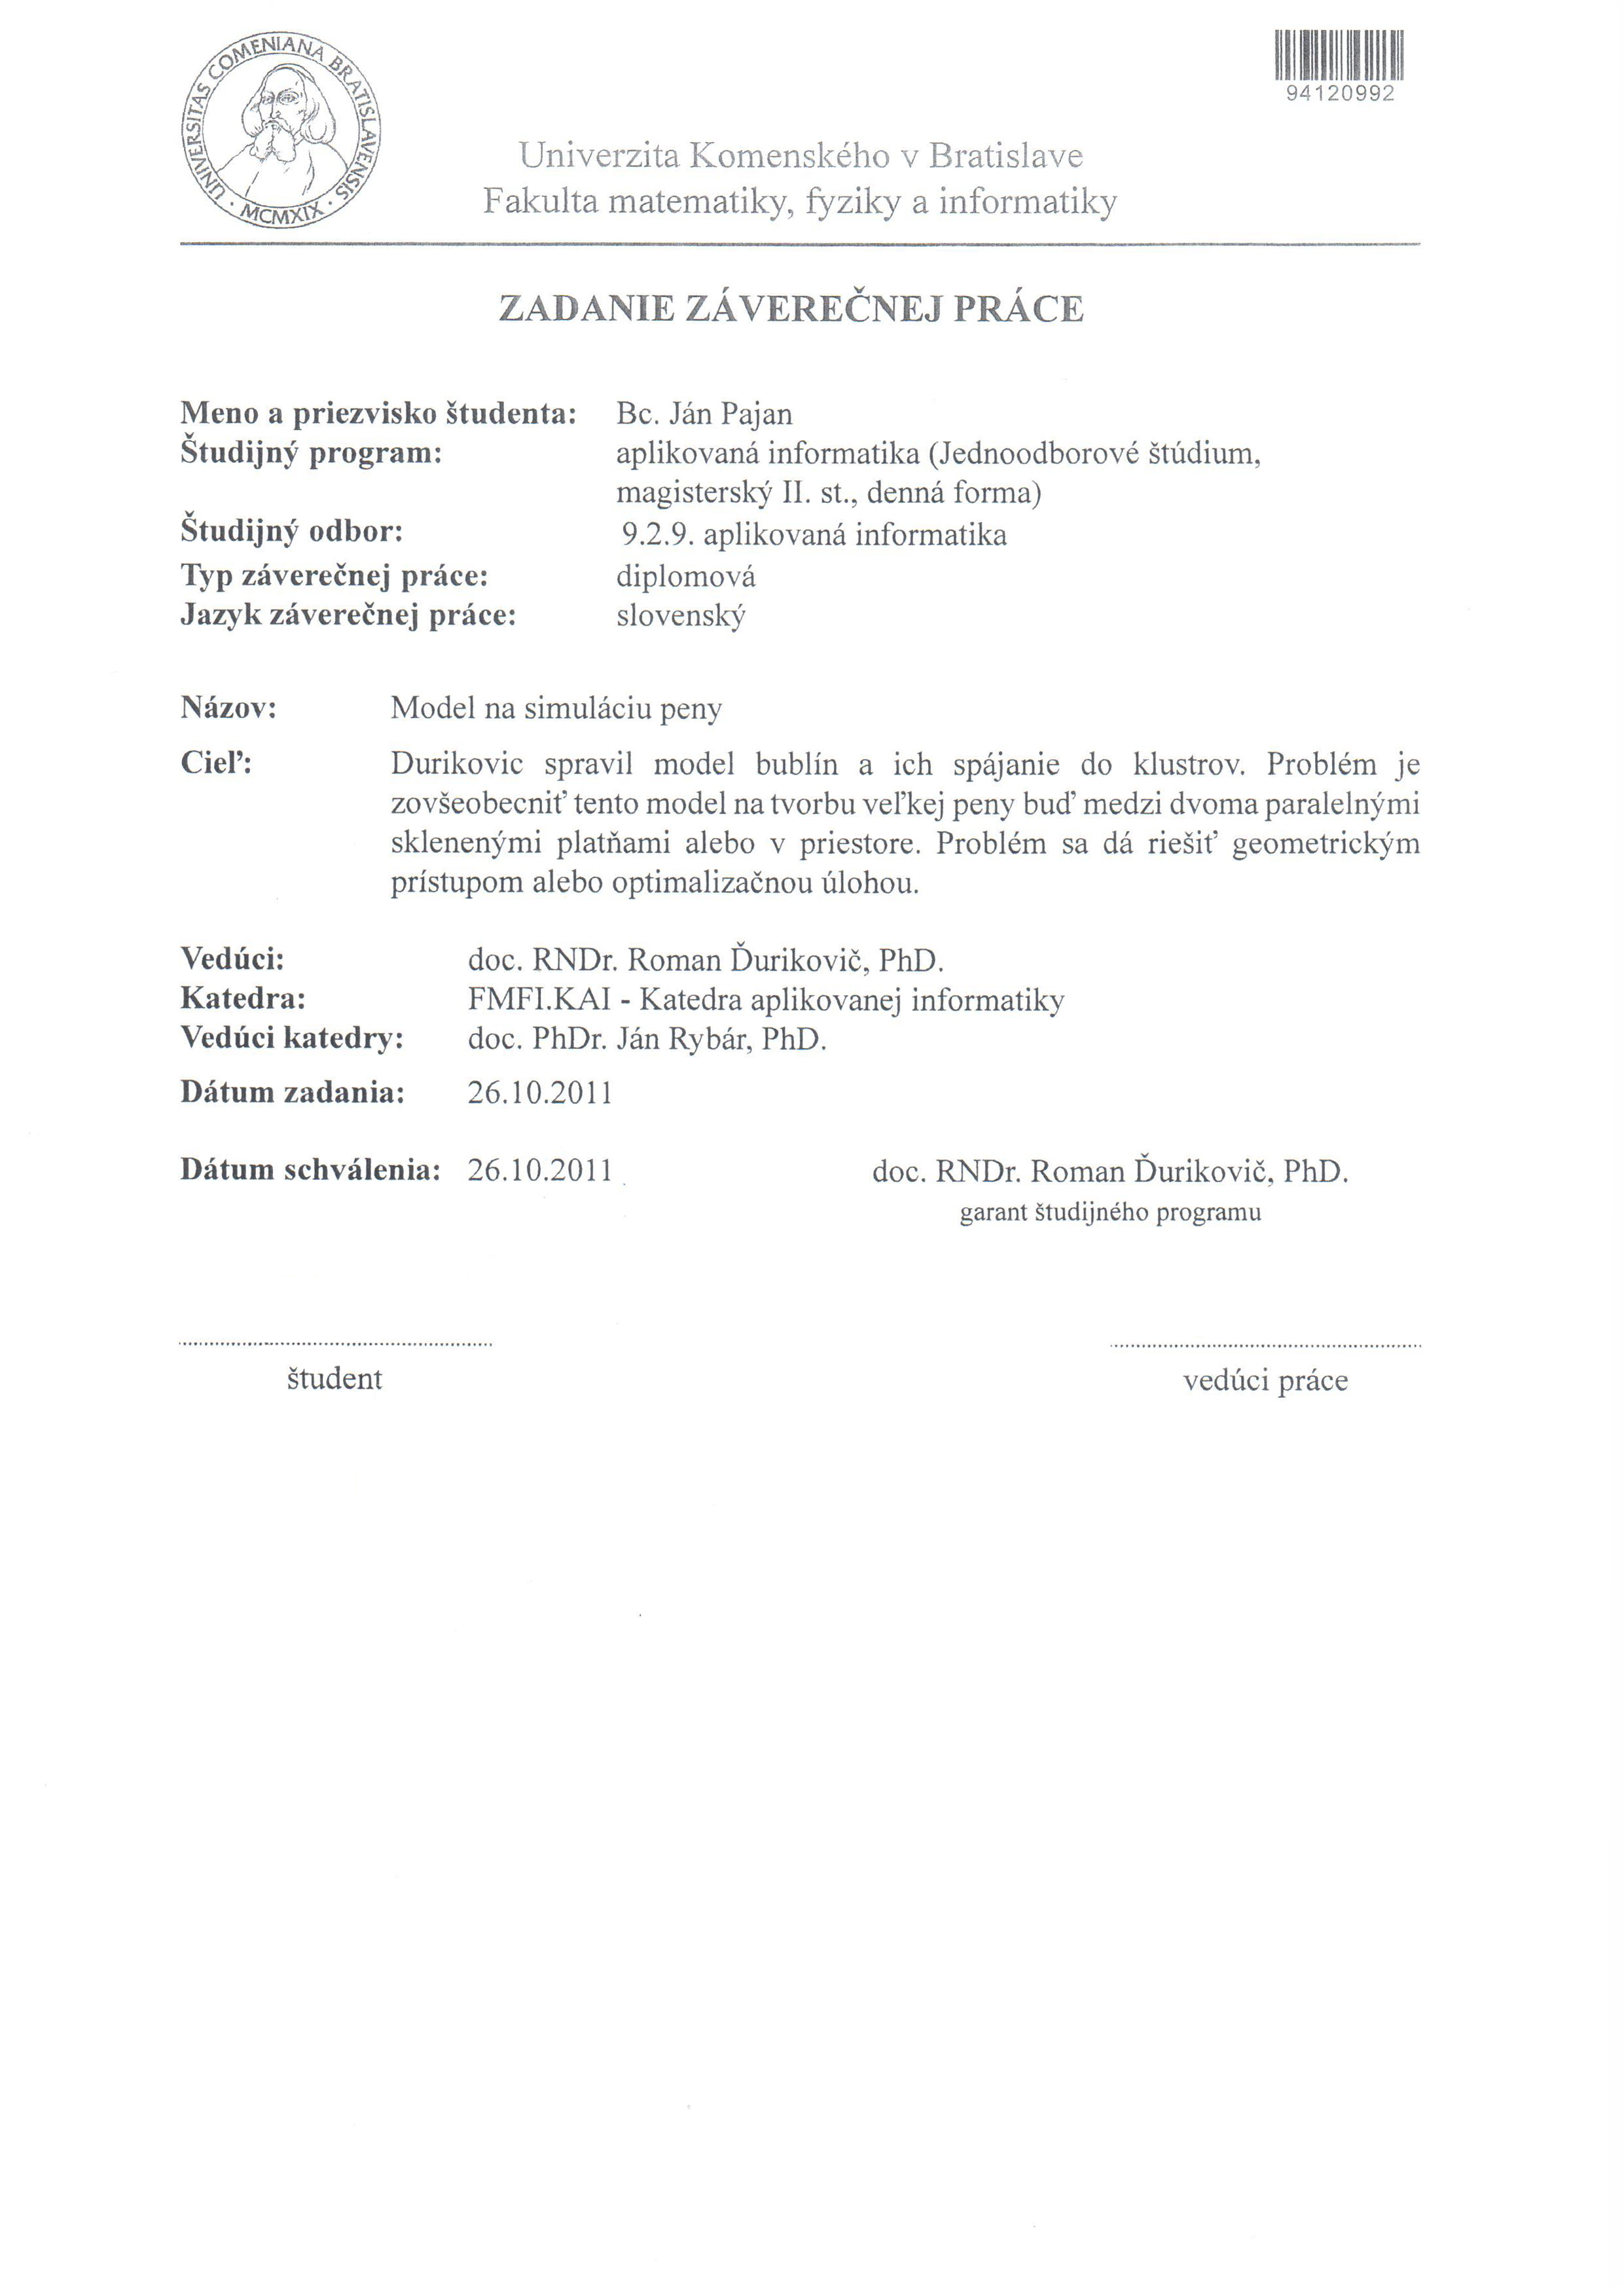
\includegraphics[width=\paperwidth]{images/zadaniedp}}
\label{img:zadanie}
\end{center}
\end{figure}

{~}\vspace{12cm}

\noindent
\begin{minipage}{0.25\textwidth}~\end{minipage}
\begin{minipage}{0.75\textwidth}
Čestne prehlasujem, že túto diplomovú prácu som vypracoval samostatne len s použitím uvedenej literatúry a za pomoci konzultácií u môjho školiteľa.
\newline \newline
\end{minipage}
\vfill
~ \hfill {\hbox to 6cm{\dotfill}} \\
\mfplacedate \hfill \mfauthor
\vfill\eject 
% koniec prehlasenia

\chapter*{Poďakovanie}\label{chap:thank_you}
Touto cestou by som sa chcel v prvom rade poďakovať môjmu školiteľovi doc. RNDr. Martinovi Homolovi, PhD. za jeho cenné rady a usmernenia, ktoré mi veľmi pomohli pri riešení tejto diplomovej práce. 
\vfill\eject 
% koniec podakovania

\chapter*{Abstrakt}\label{chap:abstract_sk}


\chapter*{Abstract}\label{chap:abstract_en}

% koniec abstraktov

\tableofcontents

\mainmatter

% treba este prejst dokument ci je kod spravne formatovany
\chapter{Úvod}\label{chap:intro}
Nejaky strucny uvod do problematiky

\chapter{Prehľad problematiky}
\section{Semantický web}
Semantický web \cite{semantic} poskytuje spoločný framework, ktorý umožňuje zdieľanie a opätovné použitie údajov v rámci aplikácií. Štandardy podporujú spoločné dátové formáty a protokoly, kde najpodstatnejším je Resource Description Framework (RDF). Prvýkrát pojem Semantický web zaviedol Tim Berners-Lee a popisoval "dátový web", ktorý môže byť strojovo čitateľný. Zámerom je zvýšiť použiteľnosť webu a jeho prepojených zdrojov vytvorením sémantického webu. Semantický web má vrstvovú štruktúru ako si môžeme všimnúť na obrázku 2.1. Jednotlivé údaje sú potrebné až vo vyšších vrstvách. XML vrstva zaručuje, že môžeme spájať Semantický web s inými normami založenými napríklad na XML, ktorá je rozšírená a podporovaná a RDF dáta sa v nej dajú dobre prenášať, spracovávať a uchovávať. RDF a RDFS vrstva definuje typ zdrojov. Ontologická vrstva podporuje vývoj ontológií, vďaka ktorým môžeme definovať vzťahy medzi rôznymi pojmami.

\assignment{MH: \UP Toto trochu povrchne: (1) Ucelom SW nie je vyssia pouzitelnost webu (to je nepresne), ale je to lepsia pristupnost informacii publikovanych na webe pre strojove spracovanie. (2) Ak chces popisovat vrstvy SW podla tohto diagramu, bolo by dobre keby si popisal vsetky vrstvy -- U XML by som sa obmedzil na to, ze je to proste dobry format pre textovu reprezentaciu dat v suboroch a pre ich vymenu medzi softvermi -- toto vsak uz je dnes prekonane, uz vymiename SW data aj ako JSON, embedujeme ich do HTML5 (chcelo by to poznamku) -- O RDF a RDFS si vlastne nic uzitocne (z coho citatel nieco vyrozumie) nepovedal -- no a ostatne vrstvy si uplne preskocil}

\begin{figure}
\makebox[\textwidth]{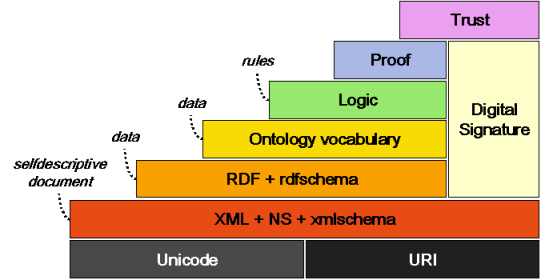
\includegraphics[scale=0.7]{images/semantic_web}}
\label{fig:semantic_web}
\caption{Semantic Web - vrstvy.\\Zdroj: \cite{semanticweb}}

\end{figure}


Text uvedený nižšie popisuje niekoľko technológií, ktoré sú potrebné pre tvorbu sémantického webu.

\subsection{Linked Data}

\assignment{MH: \DOWN Tato sekcia je celkom fajn ale chybalo mi trochu
premostenie od SW -- linked data bola iniciativa, ze ked uz SW formaty mame,
podme v nich aj data zverenjnovat}

\minor{MH: Inak ked uz si sa rozhodol pisat po slovensky, mal by si pouzivat aj
slovensku terminologiu (co je celkom peklo) -- ale teda Linked Data su
\emph{prepojene data}, LD network je \emph{siet prepojenych dat} -- ludia to takto pouzivaju}

Linked Data \cite{linkeddata} je metóda zverjňovania štrukturovaných dát. Ich hlavným cieľom je poprepájať existujúce databázy (primárne písané v RDF formáte), medzi rôznymi údajmi a umožniť ľuďom zdielať štrukturované dáta na webe pomocou HTML. Časť vízie do budúcna je, aby sa Internet stal globálnou databázou. Princípy Linked Data prvýkrát načrtol Tim Berners-Lee. Popísal 4 pravidlá pre zverejňovanie dát na webe:
\begin{enumerate}
  \item používať URI ako názvy objektov, ktoré sú identifikátormi informácie, jej umiestnenia a ďalších vlastnotí,
  \item používať HTTP URI, aby si ich ľudia vedeli pozrieť,
  \item uvádzať informácie o tom, čo názov identifikuje pri vyhľadávaní pomocou otvorených štandardov, ako sú napríklad RDF alebo SPARQL,
  \item pri publikovaní údajov na webe, zahrnúť odkazy aj na iné URI, aby sa dalo objavovať viac vecí.
\end{enumerate}
Sú známe aj ako Linked Data princípy.

\assignment{MH: Tu mi chyba informacia, ze sa tato inciativa ujala, a ze vdaka
tomu vznikla na webe tzv. siet prepojenych dat, ktora obsahuje obrovske mnozstvo
datovych zdrojov a nieco viac o tej sieti.}


\subsection{Ontológie}

\assignment{MH: Predpokladam, ze o ontologiach budeme pisat o znacny kus viac a
podrobnejsie\ldots Mozes vychadzat z mojej prednasky ale tiez napr z uvodnej
kapitoly \emph{Handbook on Ontologies}}

\overview{MH: Pozn.\ k strukture prace: Bolo by lepsie, keby \emph{Prehlad problematiky} bola cast \texttt{\textbackslash{}part\{\}}, \emph{Semanticy web} samostatna kapitola\texttt{\textbackslash{}chapter\{\}}, no a potom si myslim, ze \emph{Ontologie} by tiez mali mat vlastnu kapitolu, ktora bude nasledovat hned po SW. Tretou kapitolou by potom mohol byt prehlad ontologii z oblasti bezpecnosti, co by uz do prehladu problematiky mohlo aj stacit}

Výraz ontológia \cite{ontologies} pochádza z gréckeho slova kde '\textit{ontos}' znamená existencia a '\textit{logos}' znamená veda. Ontológia v informatike je uceleným popisom pojmov v určitej oblasti záujmu. Obsahuje určitú klasifikáciu údajov do hierarchicky usporiadaných kategórií a množinu odvodzovacích pravidiel, pomocou ktorých je možné z faktov odvodiť nové skutočnosti. Prostredníctvom ontológií je možné vytvárať spojenia v prirodzenom jazyku, vykonávať analýzu údajov a sprostredkovať výhody webu obohateného o sémantiku. Klasickými komponentami ontológií sú termy a vzťahy. Term označuje dôležitý koncept domény. Ontológia označuje kontextový vzťah za definovanými termami, zvyčajne hierarchiou tried.

\subsection{Resource Description Framework (RDF)}

RDF \cite{rdf} je štandartný model na zakódovanie metadát a ďalších informácií. Je to taktiež formát, ktorý bol navrhnutý a štandardizovaný na reprezentáciu dát pre sémantický web. Zdroje týchto dát sú väčšinou webové zdroje, ktoré môžu byť čokoľvek, napríklad dokumenty, ľudia, fyzické objekty, atď. Taktiež poskytuje spoločný framework na vyjadrenie informácií a možnosť zdieľať ich medzi softvérmi, bez straty ich hodnoty. Dáta sa uchovávajú v Triple Store databázach, ktorých formát je striktne daný. Výhodou je, že dáta môžu byť spracované aj softvérmi, pre ktoré dané dáta neboli vytvorené.

\assignment{MH: \UP Na co RDF sluzi sa uz citatel dozvedel v skorsich castiach
(ked to tam lepsie ozrejmis). Niektore veci, ktore tu \UP pises su nepresne
(napr. to o tych metadatach a ``dalsich informaciac'' alebo o zdrojoch. Tiez o Triple Stores predbiehas, budes o tom pisat neskor\ldots Asi by som to tu skratil a len by som nadviazal, ze RDF je zakladny datovy format pre SW a tu ho popiseme\ldots}

\assignment{MH: \DOWN Zvysok ide dobrym smerom, je to presne to, co by som si predstavoval, ze tu budes pisat, len by som to chcel vidiet mozno trochu pomenej, podrobnejsie, systmatickejsie prebrate\ldots Na vacsom priestore, mozno postupne ten priklad budovat\ldots Vysvetlit na nom vsetky zakladne moznosti RDF}


RDF súbor je taký dokument, ktorý ukladá RDF grafy do špecifického formátu serializácie pre RDF, ako sú napríklad N-Triple, TURTLE, RDF/XML a mnohé ďalšie. RDF bol postavený na myšlienke vytvárať údaje vo forme predmet-predikát-objekt, ktorý sa volá "triple", ďalej len trojica. Trojica je základná stavebná jednotka akejkoľvek množiny dát zapísaných v RDF. Tieto údaje sú reprezentované ako orientované grafy. Predmet a objekt predstavujú vrcholy a predikát je orientovaná hrana medzi nimi. Predmet môže byť použítý aj ako objekt v inej trojici. Týmto spôsobom sa trojice prepájajú a vzniká z nich grafová databáza. Predmet je vždy definovaný ako URI a popisuje zdroj informácie. Objekt môže byť taktiež nejaké URI popisujúce zdroj, ale taktiež to môže byť primitívna hodnota ako napríklad string, integer, date, atď. Predikát popisuje, aký vzťah alebo rola medzi predmetom a objektom existuje. Predikát je vždy reprezentovaný ako URI, ktoré pochádza z ontolológií (kolekcie viacerých URI).


Na uľahčenie ukladania a čitateľnosti dát sa využívajú takzvané prefixy, ktoré sú preddefinovaním základných URI, do ktorých sa dodáva zvyšná hodnota URI pomocou dvojbodky, ako je to uvedené v nasledujúcom príklade a graficky znázornené v obrázku 2.2.
\begin{verbatim}
@prefix  rdf: <http://www.w3.org/1999/02/22-rdf-syntax-ns> .
@prefix	 dbr: <http://dbpedia.org/resource/> .
@prefix 	 dbo: <http://dbpedia.org/ontology/> .
@prefix  dbp:<http://dbpedia.org/property/> .

dbr:Bratislava dbo:highestPlace dbr:Devínska_Kobyla .
dbr:Bratislava rdf:type dbo:City .
dbr:Bratislava dbo:country dbr:Slovakia .
dbr:Devínska_Kobyla dbo:locatedInArea dbr:Slovakia .
dbr:Slovakia dbp:drivesOn "right" .
dbr:Slovakia dbo:longName "Slovak Republic"@en .
\end{verbatim}

\begin{figure}[h]
\makebox[\textwidth]{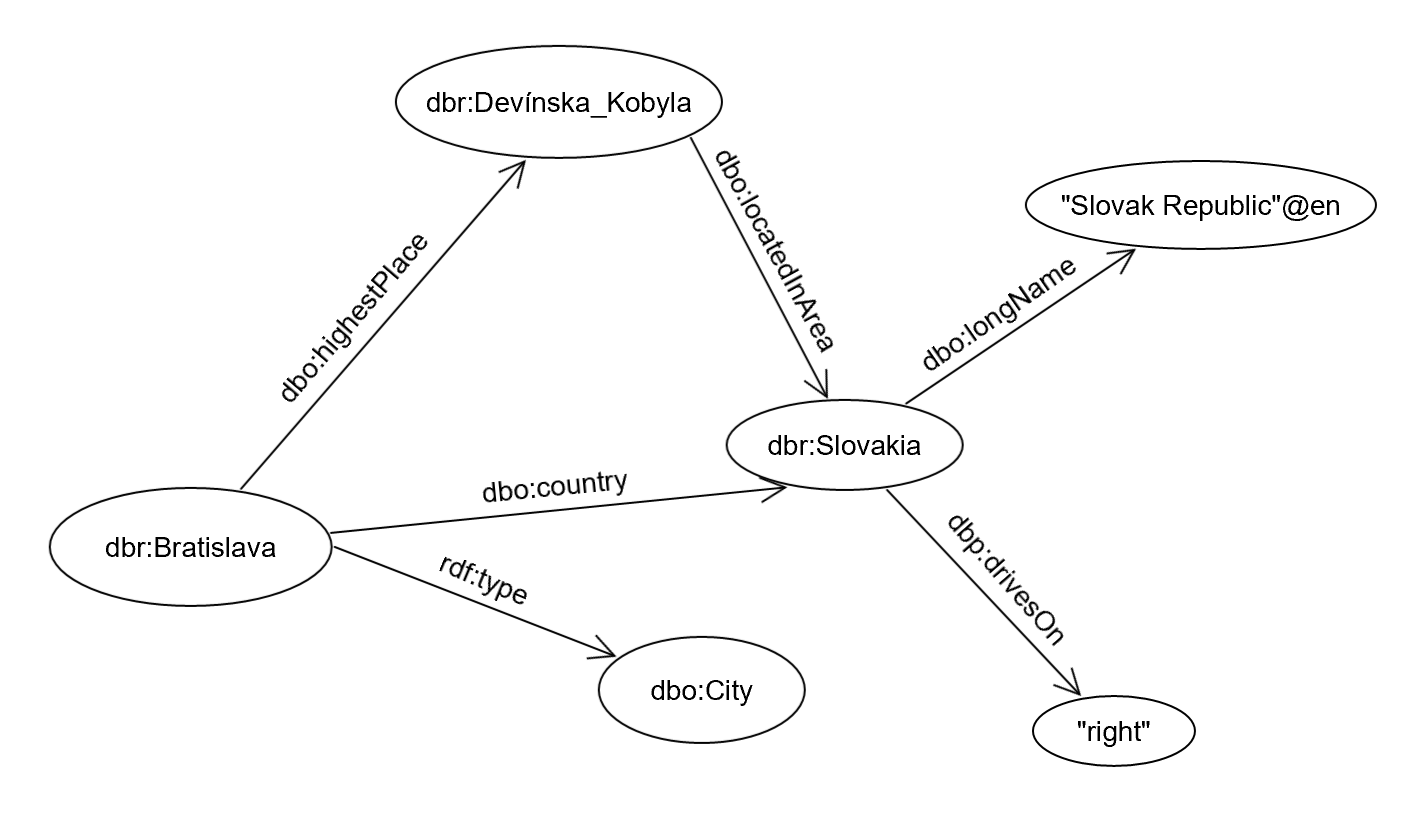
\includegraphics[keepaspectratio=true,scale=0.7]{images/triple_example}}
\label{fig:semantic_web}
\caption{Príklad grafovej databázy.}
\end{figure}

\subsection{Triple Store}
Triple store \cite{triplestore} alebo RDF store slúži na uchovávanie a načítavanie trojíc z databázy prostredníctvom sémantických dopytov. Dopyty sú robené v jazyku SPARQL. Dáta ukladá v grafovej databáze, ktorá ukladá sémantické fakty. \cite{triplestore}


Implemetntácie Triple Store sú rôzne. Môžu byť postavené na tabuľkovej reprezentácií, kde máme tabuľku s tromi stĺpcami, kde každý stĺpec predstavuje jedno z hodnôt trojice. Následné SPARQL dopyty sa transformujú na SQL dopyty. Taktiež sa môžu skladať z dokumentových databáz, kde zdrojovými súbormi môžu byť všetky tie, ktoré dodržiavajú definovanú RDF syntax.

\assignment{MH: \UP Toto zrejme nie je typicka implementacia. Ked chces o tom
pisat, mozes si to skusit niekde nastudovat. (Mozes samozrejme spomenut aj tuto
moznost, ale nie ako jedinu.)}
\overview{MH: Inak zrovna pre tuto pravcu mozno nie su triple
stores az take nosne, mozno by sme sa im v prehlade ani venovat nemuseli --
aspon zatial, mozeme neskor doplnit ak by bolo treba}

V triple Store je aj možnosť pomenovávať jednotlivé časti grafov. Napríklad ak si chceme celý Triple Store rozdeliť na časti, pomenujeme graf, a pomocou tohoto mena definujeme trojice. Z trojíc sa stávajú štvorice, kde jedným prvkom je názov grafu, pod ktorý trojica spadá.

\subsection{SPARQL}

\overview{MH: Podobne ako v pripade triple stores, zatial by som to neriesil, mozno to pre nas nebude dolezite. Ak ano, potom by som to doplnil (a rozpisal viac dopodrobna)}

SPARQL \cite{sparql} je dopytovací jazyk pre RDF databázy, ktorý umožňuje získavanie a manipuláciu s databázou. Bol vytvorený skupinou DAWG, ktorá je súčasťou W3C a je uznávaný ako kľúčová technológia sémantického webu. 


\quad Ak by sme porovnali SPARQL s dopytovacím jazykom pre relačné datábazy, napr. SQL, zistíme, že sú si podobné v kľúčových slovách, ako sú napr. SELECT, WHERE, FROM atď. SPARQL dopyt využíva trojice ako základný prvok, kde predmet, predikát alebo objekt môžu byť premenné. Dopyt sa robí nad dátovou kolekciou RDF, čo je množina dokumentov, patriaca pod určitý koncový bod - '\textit{endpoint}'. Je to dopytovací jazyk, ktorý z orientovaného ohodnoteného grafu zisťuje hodnoty jednotlivých vrcholov a hrán, ktoré sú výstupnými parametrami dopytu.


\begin{verbatim}
@prefix	 dbr: <http://dbpedia.org/resource/> .

SELECT ?predicate ?object WHERE {
  dbr:Bratislava ?predicate ?object .
}
Výsledok dopytu:
+------------------+---------------------+
| ?predicate       | ?object             | 
+------------------+---------------------+
| dbo:highestPlace | dbr:Devínska_Kobyla | 
| rdf:type         | dbo:City            | 
| dbo:country      | dbr:Slovakia        | 
+------------------+---------------------+
\end{verbatim}


Príklad dopytu nad databázou uvedenou vyššie, spúšťame nad endpointom DBPedia a výsledok je len zlomkom z toho, čo nám skutočne vráti: Chceme získať všetky údaje o Bratislave.


Okrem operácie SELECT poznáme aj ďalšie typy dopytov. ASK je dopyt, ktorý nám vracia pravdivostnú hodnotu pre daný dopyt. Vieme ním napríklad zistiť či sa v našom grafe nachádza mesto Bratislava. Taktiež poznáme dopyt DESCRIBE, ktorý vracia RDF graf opisujúci jednotlivé vlatnosti výsledných hodnôt dopytu. Ako posledný typ dopytu je CONSTRUCT, ktorý vracia nový RDF graf podľa predlohy vytvorenej v hlave dopytu.

\backmatter

\nocite{*}
\bibliographystyle{alpha}
\bibliography{references}

\listoffigures

\end{document}
